\documentclass[referee, pdflatex, sn-mathphys-num]{sn-jnl}

\usepackage{hyperref}
\usepackage{subfigure}
\usepackage{graphicx} 
\usepackage{amsmath,amsfonts,amssymb,amsthm,mathtools}
\usepackage{icomma}
\usepackage[english]{babel}
% tables
\usepackage{array,tabularx,tabulary,booktabs}
\usepackage{multirow}
\usepackage{diagbox}

\theoremstyle{definition}
\newtheorem{Def}{Definition}
\theoremstyle{plain}
\newtheorem{Lem}{Lemma}
\newtheorem{Th}{Theorem}

\newcommand{\bz}{\ensuremath{\mathbf{z}}}

\begin{document}
	
	\title{Time series classification approaches through NeuralODE}
	
	\author*[1]{\fnm{Kirill} \sur{Semkin}}\email{semkin.ki32@gmail.com}
	\author*[2]{\fnm{Vadim} \sur{Strijov}}\email{strijov@forecsys.ru}
	
	\affil*[1]{\orgname{MIPT} \orgaddress{\city{Moscow}} \country{Russia}}
	\affil*[2]{\orgname{MIPT} \orgaddress{\city{Moscow}} \country{Russia}}
	
	\keywords{time series; classification; dynamical systems; NeuralODE; inertial measurement unit}
	
	\maketitle
	
	\begin{abstract}
		
		The task of time series classification is to assign class label to given time series. The number of classes is fixed. It is assumed that each class corresponds to some dynamical system. Each system generates phase trajectories within some probabilistic model. These trajectories are then mapped into empirical observations. The paper investigates how to restore dynamical systems out of experimental data using NeuralODE. We consider fixed and bayesian approaches to defining dynamical systems' parameters. Two classification principles are introduced: bayesian testing and transition to dynamical system's parameters space. Taken's theorem is used to approximate true phase trajectories. At last, time series from inertial measurement unit are classified using given techniques and compared with other machine learning models.
		
	\end{abstract}
	
	\section{Introduction}\label{Intro}
	
		The paper introduces and analyzes methods for time series classification. By \emph{time series} we understand samples of some \emph{stochastic process}. Consider $x(t)$ to be stochastic process defined on $t \in [0, T]$. Take increasing time stamps $0 \le t_1 < \ldots < t_n \le T$ and define time series as $x_i := x(t_i), \, i \in 1 \ldots n$. So time series are stochastic variables by definition. \emph{Classification} of time series on $M$ classes is a process of assigning a \emph{label} $y \in 1 \ldots M$ to a given time series $x_i$.
		
		% Applications
		Time series classification finds a lot of applications. It is used in medicine to detect arrhythmias or other heart conditions by EEG~\cite{application_eeg_1}. Or to identify seizures and sleep stages from brainwave data~\cite{application_eeg_2}. In speech and audio processing it is used to recognize human emotions from speech signals~\cite{application_sound_1} or bird species from audio recordings~\cite{application_sound_2}. Other fields of application are human activity recognition from wearable sensors~\cite{application_hac} and weather forecasting~\cite{application_weather}. The latter two will be explored in the paper's experiment later.
		
		% Methods from literature review
		There are many methods for time series classification in the literature. \emph{Distance-based} approaches rely on measuring similarity between time series using distance metrics. The metric can be defined using Dynamic Time Warping~\cite{dtw} and the k-Nearest-Neighbors (k-NN) classifier can be used then~\cite{knn_dtw}. \emph{Feature-based} approaches extract finite set of statistical~\cite{stat_feat_1, stat_feat_2} or spectral~\cite{fouirer_feat} features from time series for further classification. \emph{Deep learning} approaches uses neural networks to automatically learn time series features from raw train data. Convolutional neural networks~\cite{application_eeg_1, application_eeg_2}, recurrent neural networks (RNN)~\cite{lstm_feat} or their combination~\cite{application_sound_1, application_hac, application_weather} are designed to process sequential data like time series. Classification with the RNN will be compared to our method in the experiment section.
		
		The underlying mathematical model for time series in the paper is a \emph{dynamical system}. By this we understand a time-invariant \emph{ordinary differential equation (ODE)} of the form
		\begin{equation}\label{eq:lat_dyn}
			\begin{cases}
				\bz = f(\bz), \\
				\bz(0) = \bz_0,
			\end{cases}
		\end{equation}
		where $\bz \in \mathbb{R}^m$, $f(\bz): \mathbb{R}^m \to \mathbb{R}^m$ is a \textit{vector field}, $\bz_0$ is a \textit{starting point}. \textit{Phase trajectory} $\bz(t)$ is a solution of (\ref{eq:lat_dyn}) for $t \in [0, T]$. Note that the phase trajectory is not directly observed so we call the dynamical system \emph{latent}. Next, introduce an \emph{observation function} $\phi: \mathbb{R}^m \to \mathbb{R}$. It maps phase trajectory to intermediate deterministic representation $y(t) = \phi \big( \bz(t) \big)$. Finally, we introduce a stochastic field $h:  \mathbb{R} \times [0, T] \to \Omega$. It maps intermediate representation to observable stochastic process $x(t) = h(y(t), t)$ introduced at the begging. The process takes random variables on a probability space $(\Omega, \mathcal{F}, \mathbb{P})$. The stochastic field $h$ can be treated as adding noise to original observations $y(t)$.
		
		% TODO: insert our time series model illustration
		
		The reason for introducing an intermediate process $y$ is to be able to use Takens theorem \cite{takens2006detecting}. It basically states that if can estimate $y(t)$ from $x(t)$ then we are able to reconstruct latent phase trajectory $z(t)$.  It is important for classification because we \emph{associate each class label $y$ with some dynamical system} $f_y(\cdot), \, y \in 1 \ldots M$. Illustration of the theorem is on the Fig.~\ref{fig:takens}. If we know $f_y(\cdot)$ for every $y$ and $z(t)$ is given, we can inference the dynamical system that generated this phase trajectory. Thus we can inference class label and perform classification.
		
		\begin{figure}[h]
			\centering
			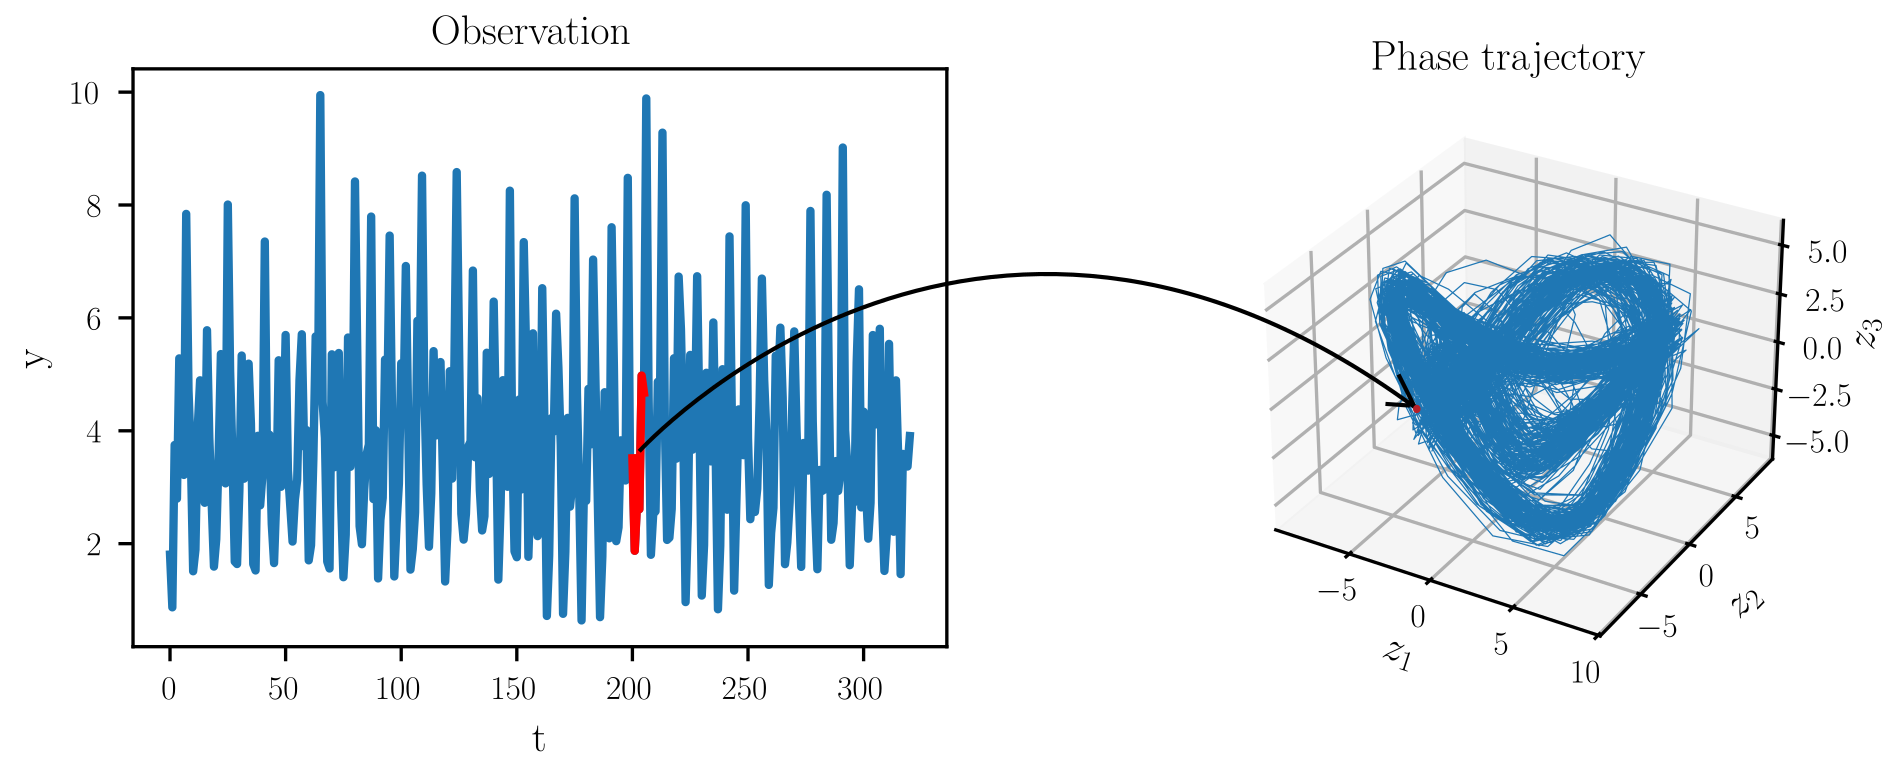
\includegraphics[width=\textwidth, keepaspectratio]{takens}
			
			\caption{Application of the Takens theorem. On the left are observations $y(t)$. To build a point of the latent phase trajectory $\bz(t)$ we must take several lagged observation values (colored in red), e.g. $\bz(t) = \big( y(t-1), y(t-2), y(t-3) \big)^{\text{T}}$.}\label{fig:takens}
		\end{figure}
		
		% Contains NODE review
		When we don't know vector fields $f_y(\cdot)$ we approximate them from labeled trajectories. The algorithm for approximation we will use is Neural Ordinary Differential Equations (NODE)~\cite{node}. It allows to use gradient optimization when an optimized objective depends on ODE trajectories. There are plenty of papers using NODE for regression tasks. For example, NODE are used in the context of physics-informed ODE~\cite{LAI2021116196, phys_informed_2} and control learning~\cite{NEURIPS2019_99a40143, node_rl}. However very few papers analyze NODE in the context of time series classification. Authors of~\cite{8892510} reinterpreted convolutional neural networks in terms of latent ODE dynamics and used it for hyperspectral image classification. Paper~\cite{node_control} interestingly formulated and solved general classification problem in terms of control theory and NODE. Our paper contributes to NODE classification in terms of latent dynamical systems for time series.
		
		% NODE's time series model critique
		Original NODE paper~\cite{node} introduced its own generative latent time-series model in its section 5. It basically uses the same latent dynamical system model as ours. Observations are generated from latent trajectories through general probability distribution. The authors then used variational autoencoder~\cite{Kingma2013AutoEncodingVB} to inference the distribution and latent vector field. We point out three drawbacks of this approach. First, it struggles to define the starting point $\bz_0$ of the latent trajectories from the observations. Authors need to introduce additional probability distribution to account for that. Second, it is not clear how introduced probability distributions should look like for particular tasks. Third, this approach does not give explicit way to reconstruct latent trajectories from the observations. Authors have to resort to variational principle~\cite{blei2017variational} and introduce additional parametric models for reconstruction. On the contrary, our time series model does not have problems with starting point and trajectory reconstruction thanks to the Takens theorem. Our general stochastic component $h(y(t), t)$ of the model only affects transition from intermediate state $y$ to observations $x$ and can be easily interpreted for particular tasks as a noise. Applying Takens theorem ideas and NODE to restore latent dynamics can be find in literature~\cite{node_takens_1, node_takens_2}. But unfortunately, it is poorly covered for machine learning applications. Our paper aims to close this gap.
		
		% TODO: insert graphical models
		
		% Classification approachess
		To build a classifier we will first introduce two probabilistic models to connect class label and dynamical system. The models will be expressed as \textit{probabilistic graphical models}~\cite{bishop}. Then, we will use bayessian classification~\cite{bishop}, variational principle~\cite{blei2017variational} or change of variables~\cite{hogg2005introduction} as means for different classification methods. They are all theoretical principles from statistics that lead to particular classifier. We will explore them later. 
		
		% About numerical approximations
		Every classification method is negatively effected by numerical approximations of solving (\ref{eq:lat_dyn}). This is because NODE is based on imprecise numerical ODE solvers~\cite{ode_solvers}. We will show how the classification quality decreases depending on the length $n$ of the latent trajectory $\bz(t_i)$. So limited trajectory length is an explicit constraint of our approach. Another reason for this limit is inaccurate vector field reconstruction from the labeled data. We will include it into the analysis as well. Finally, the latent dynamical system itself may be inadequate model for the whole time series. But it can fit time series locally. So we have limit on the trajectories again. Let's call the maximum trajectory length that can be properly classified as \emph{forecasting horizon} and denote it as $K$. More formal definition will be given later in the paper. If we have trajectory to be classified longer than the forecasting horizon, the general solution we suggest is to split the trajectory on chunks of the length $K$. We will show how to adapt the classification methods for this case. Note that usually numerical approximation are not accounted in NODE applications but for us they are crucial and must be analyzed.
		
		% TODO: experiment and layout
		% WHEN:  the experiment is ready
		
		
		
		
		
		
		
		\bibliography{lit.bib}
	
 \end{document}